\chapter{Dekoder: od map prawdopodobieństw do listy nut}\label{rozdz:dekoder}

\section{Sieć nie zwraca nut}

Sieć zwraca \emph{mapy}: dla każdej klatki i półtonu liczby $p_\mathrm{on},p_\mathrm{fr},p_\mathrm{off}\in(0,1)$. My chcemy listę nut (wysokość, początek, koniec, struna). Przejście od map do listy robi \emph{dekoder} --- zwykły algorytm, bez parametrów uczonych gradientem
(jest nieróżniczkowalny: zawiera progi i wybór maksimów, zob.\ rys.~\ref{rys:funkcje-pomocnicze}c). Jego progi to \emph{hiperparametry} i trzeba je dobrać osobno (na walidacji).

Po tym rozdziale umiesz: (i)~przeprowadzić dekoder ręcznie dla jednego półtonu, (ii)~wybrać strunę nuty z mapy tabulatury, (iii)~uzasadnić, że przeszukiwanie progów po współrzędnych nie pogarsza celu, (iv)~odczytać, co zmienia dostrojenie progów.

\section{Algorytm dla jednego półtonu}

Dekoder działa na każdy półton $s$ osobno, przeglądając klatki $t=0,1,\dots,T-1$ i pamiętając stan: klatkę początku \texttt{start}, ostatnią klatkę brzmienia \texttt{last} i licznik przerwy \texttt{gap}.

\haslo{pik}
\begin{definicja}[Pik początku]\label{def:pik}
Klatka $t$ jest \emph{pikiem początku} w półtonie $s$, gdy $p_\mathrm{on}(t,s)\ge\theta_\mathrm{on}$ jest lokalnym maksimum ($p_\mathrm{on}(t,s)\ge p_\mathrm{on}(t-1,s)$ i $>p_\mathrm{on}(t+1,s)$) oraz $p_\mathrm{fr}(t,s)\ge\theta_\mathrm{on,fr}$.
Analogicznie \emph{pik końca}: lokalne maksimum $p_\mathrm{off}\ge\theta_\mathrm{off}$.
\end{definicja}

\textbf{Reguły} (dla klatki $t$ po kolei):
\begin{enumerate}
\item \emph{Początek.} Na piku początku zaczynamy nową nutę ze \texttt{start}$=t$ (jeśli trwała poprzednia, najpierw ją kończymy: to ponowne szarpnięcie). Gdy nie ma piku, a nie ma trwającej nuty, nuta może wystartować, jeśli $p_\mathrm{fr}\ge\theta_\mathrm{start}$ przez $n_\mathrm{min}$ klatek (w modelu końcowym wyłączone: $\theta_\mathrm{start}=1{,}01>1$).
\item \emph{Trwanie.} Dopóki $p_\mathrm{fr}(t,s)\ge\theta_\mathrm{fr}$, nuta trwa (\texttt{last}$=t$, \texttt{gap}$=0$); w przeciwnym razie \texttt{gap}$\mathrel{+}=1$, a gdy \texttt{gap}$>g_\mathrm{max}$, nuta się kończy.
\item \emph{Koniec z głowicy.} Jeśli $t>$\texttt{start} jest pikiem końca, nuta kończy się w $t$.
\end{enumerate}
\textbf{Wynik nuty:} wysokość $36+s$, początek $t_0=\max(0,\tau_\text{start})$, koniec $t_1=\max\big(t_0+d_\mathrm{min},\ \tau_\text{last}+\tfrac12\Delta\big)$ (gdzie $\tau$ to środek klatki, $\Delta=23{,}2\ms$), pewność $=$ średnie $p_\mathrm{fr}$ w klatkach nuty.
Nuty krótsze niż $n_\mathrm{min}=2$ klatki odrzucamy; dwie nuty tej samej wysokości o początkach bliższych niż $\theta_\mathrm{merge}$ scalamy w jedną.

\begin{przyklad}[Jedna nuta ręcznie]\label{prz:dekoder-reczny}
Półton E4 ($s=28$), progi dostrojone ($\theta_\mathrm{on}=0{,}6$, $\theta_\mathrm{on,fr}=0{,}1$, $\theta_\mathrm{fr}=0{,}6$, $\theta_\mathrm{off}=0{,}8$). W klatkach $33$--$37$:
$p_\mathrm{on}=(0{,}05;\,0{,}30;\,0{,}85;\,0{,}40;\,0{,}05)$, a $p_\mathrm{fr}=(0{,}2;\,0{,}7;\,0{,}9;\,0{,}9;\,0{,}9)$ i dalej $0{,}9$ do klatki $53$. W klatce $35$: $p_\mathrm{on}=0{,}85\ge0{,}6$, większe od sąsiadów ($0{,}30$ i $0{,}40$), a $p_\mathrm{fr}=0{,}9\ge0{,}1$ --- to pik: początek nuty.
Czas: $t_0=\tau_{35}=(35\cdot256+2048)/11\,025=0{,}998$ s. Dalej $p_\mathrm{fr}\ge0{,}6$, więc nuta trwa. W klatce $53$ niech $p_\mathrm{off}=0{,}9\ge0{,}8$ (lokalne maksimum): koniec, $t_1=\tau_{53}+\tfrac12\Delta=1{,}4164+0{,}0116=1{,}428$ s.
Wynik: nuta (E4; $0{,}998$ s; $1{,}428$ s). Ten sam wynik daje kod repozytorium.
\end{przyklad}

\begin{figure*}[ht]
\centering
\begin{tikzpicture}[>=Stealth,node distance=4.5mm,font=\footnotesize]
  \tikzset{st/.style={draw,rounded corners=2mm,thick,minimum height=8mm,minimum width=17mm,align=center,fill=white},
           eti/.style={font=\scriptsize,midway,fill=white,inner sep=1pt}}
  \node[st] (cisza) {cisza};
  \node[st,right=22mm of cisza,fill=blue!8!white] (gra) {nuta trwa};
  \node[st,right=22mm of gra] (kon) {zapis\\nuty};
  \draw[->,thick] (cisza) -- node[eti,above=1mm]{pik $p_\mathrm{on}$} (gra);
  \draw[->,thick] (gra) -- node[eti,above=1mm]{pik $p_\mathrm{off}$} node[eti,below=1mm]{lub \texttt{gap}$>g_\mathrm{max}$} (kon);
  \draw[->,thick] (kon.south) -- ++(0,-6mm) -| (cisza.south);
  \draw[->,thick] (gra.north) -- ++(0,5mm) -| node[eti,pos=0.25,above=1mm]{pik $p_\mathrm{on}$: ponowne szarpnięcie} (gra.north east);
\end{tikzpicture}
\caption{Maszyna stanów dekodera dla jednego półtonu. Z ciszy wychodzi się na piku początku; nuta trwa, dopóki $p_\mathrm{fr}\ge\theta_\mathrm{fr}$; kończy ją pik końca albo przerwa dłuższa niż $g_\mathrm{max}$ klatek; nowy pik początku w trakcie nuty kończy ją i zaczyna następną.}
\label{rys:dekoder-stany}
\end{figure*}

\begin{intuicja}
Początek bierzemy z \emph{pików} głowicy początku, bo ona jest ostra (rzadkie etykiety, miękkie $0{,}4$ obok); trwanie z głowicy „brzmi”, bo ona jest szeroka; koniec z piku końca, a gdy go nie ma --- z tego, że „brzmi” opadło. Trzy głowice dają trzy niezależne wskazówki, dekoder je łączy.
\end{intuicja}

\begin{naliczbach}
Przypadek bez piku końca: jeśli w klatce $53$ jest $p_\mathrm{off}=0{,}3<0{,}8$, a po klatce $53$ $p_\mathrm{fr}=0{,}1<0{,}6$, to w klatkach $54,55,56$ licznik \texttt{gap} rośnie do $3>g_\mathrm{max}=2$ i nuta się kończy z \texttt{last}$=53$: koniec jest ten sam, $1{,}428$ s.
Przypadek za niskiego piku: gdyby $p_\mathrm{on}$ w klatce $35$ wynosiło $0{,}55<0{,}6$, dostrojony dekoder \emph{zgubi nutę} (bo $\theta_\mathrm{start}$ jest wyłączony), a dekoder domyślny ($\theta_\mathrm{on}=0{,}5$, $\theta_\mathrm{on,fr}=0{,}3$) znajdzie ją.
\end{naliczbach}

\begin{figure*}[ht]
\centering
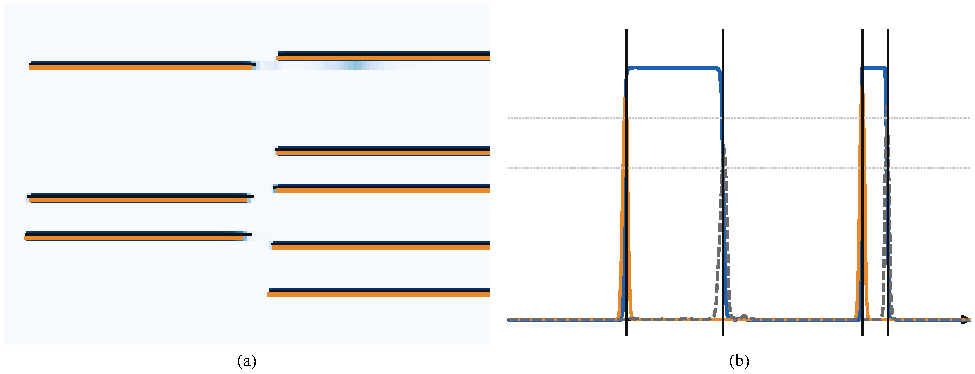
\includegraphics[width=\linewidth]{figures/dekoder-model.pdf}
\caption{Dekoder na wyjściach prawdziwego modelu Gen~6 (syntetyczne nagranie z $15$ nutami). (a) Mapa $p_\mathrm{fr}$ (jasność), fragment $110$ klatek i półtony $4$--$39$; czarne kreski --- prawdziwe nuty, pomarańczowe --- nuty z dekodera (każda para blisko siebie; największy błąd początku $18{,}7\ms$).
(b) Trzy głowice dla jednego półtonu z dwiema nutami: $p_\mathrm{fr}$ (niebieska), $p_\mathrm{on}$ (pomarańczowa), $p_\mathrm{off}$ (szara przerywana) i progi $\theta_\mathrm{on}=0{,}6$, $\theta_\mathrm{off}=0{,}8$ (kropkowane poziome); czarne pionowe kreski to początki i końce nut z dekodera.}
\label{rys:dekoder-model}
\end{figure*}

\section{Wybór struny}

Dla nuty o wysokości $m$ i klatkach $\mathcal N=\{\text{start},\dots,\text{last}\}$ strunę wybiera się jako tę o największym \emph{średnim} prawdopodobieństwie właściwej klasy:
\begin{equation}
  i^\ast=\argmax_{i:\ 0\le m-o_i<20}\ \frac1{\abs{\mathcal N}}\sum_{t\in\mathcal N}p_i(t)\big[\,1+(m-o_i)\,\big].
\end{equation}

\begin{przyklad}\label{prz:wybor-struny}
Nuta $m=52$ (E3) ma trzy pozycje: struna~6 próg~12, struna~5 próg~7, struna~4 próg~2 (struny~3, 2, 1 odpadają, bo $52-55,52-59,52-64<0$). Jeśli średnie prawdopodobieństwa tych klas w klatkach nuty to $0{,}10$ (struna~6), $0{,}20$ (struna~5), $0{,}70$ (struna~4), dekoder wybiera strunę~4 (D3), próg~2. Sprawdzone kodem repozytorium.
\end{przyklad}

\section{Strojenie progów}

Progów nie da się wyznaczyć gradientem, więc dobieramy je na \emph{walidacji} (222 nagrania: 12 GuitarSet, 150 klasyki, 60 środowisk) \emph{przeszukiwaniem po współrzędnych}: dla każdego progu po kolei próbujemy siatkę wartości przy pozostałych ustalonych, zostawiamy najlepszą, i tak dwa przebiegi. Cel:
\begin{equation}
  J=100\cdot\frac{\sum_{z}w_z\,\overline{\tfrac12\big(F_\mathrm{on}+F_\mathrm{on+off}\big)}_z}{\sum_zw_z},
\end{equation}
z wagami grup $w_\mathrm{GuitarSet}=0{,}4$, $w_\mathrm{klasyka}=0{,}4$, $w_\mathrm{środowiska}=0{,}2$,
gdzie $F_\mathrm{on}$ to F1 nut, a $F_\mathrm{on+off}$ F1 nut z końcem (rozdział~\ref{rozdz:wyniki}), uśrednione po nagraniach każdej grupy $z$.

\begin{twierdzenie}[Przeszukiwanie po współrzędnych jest monotoniczne]\label{tw:wspolrzedne}
Niech siatka wartości dla każdego progu jest skończona i zawiera aktualną wartość. Jeśli w każdym kroku wybieramy wartość maksymalizującą $J$ (przy remisie --- dotychczasową), to $J$ nigdy nie maleje, a procedura kończy się po skończonej liczbie kroków.
\end{twierdzenie}
\begin{pomyslDowodu}
Aktualna wartość jest jednym z kandydatów, więc maksimum po siatce jest nie mniejsze niż dotychczasowa wartość celu.
\end{pomyslDowodu}
\begin{proof}
Niech $\vect\theta$ będzie bieżącym wektorem progów, a $G_k$ siatką dla progu $k$ z $\theta_k\in G_k$. Po kroku dla progu $k$ nowa wartość $\theta_k'$ spełnia
\begin{align*}
J(\theta_k',\vect\theta_{-k}) &= \max_{g\in G_k}J(g,\vect\theta_{-k}) && \pow{(wybór najlepszego kandydata)}\\
 &\ge J(\theta_k,\vect\theta_{-k}) && \pow{($\theta_k\in G_k$)}
\end{align*}
więc $J$ nie maleje. Liczba przebiegów jest ustalona (dwa), a każdy przebieg ma skończoną liczbę progów i skończone siatki, więc procedura się kończy. To kończy dowód.
\end{proof}

Warto pamiętać, czego twierdzenie \emph{nie} mówi: nie gwarantuje globalnego maksimum (tylko lokalne w kierunku osi) ani, że poprawa na walidacji przeniesie się na dane nowe.

\begin{table}[ht]
\centering\small
\begin{tabular}{@{}llcc@{}}
\toprule
próg & znaczenie & domyślny & dostrojony\\
\midrule
$\theta_\mathrm{on}$ & próg piku początku & $0{,}5$ & $\mathbf{0{,}6}$\\
$\theta_\mathrm{on,fr}$ & wymagane $p_\mathrm{fr}$ przy początku & $0{,}3$ & $\mathbf{0{,}1}$\\
$\theta_\mathrm{fr}$ & próg trwania nuty & $0{,}5$ & $\mathbf{0{,}6}$\\
$\theta_\mathrm{off}$ & próg piku końca & $0{,}5$ & $\mathbf{0{,}8}$\\
$\theta_\mathrm{start}$ & nuta bez piku początku & $0{,}7$ & $\mathbf{1{,}01}$ (wyłączone)\\
$g_\mathrm{max}$ & przerwa kończąca nutę [klatki] & $1$ & $\mathbf{2}$\\
$\theta_\mathrm{merge}$ & scalanie duplikatów [s] & $0{,}03$ & $\mathbf{0{,}08}$\\
\bottomrule
\end{tabular}
\caption{Progi dekodera Gen~6: domyślne i dostrojone na walidacji (plik \texttt{decode.json}). Pozostałe: $n_\mathrm{min}=2$ klatki, $d_\mathrm{min}=0{,}06$ s bez zmian.}
\label{tab:progi}
\end{table}

\textbf{Efekt.} Cel na walidacji wzrósł z $79{,}57$ do $80{,}87$. Największy wkład ($+0{,}75$) dało \emph{wyłączenie nut bez wykrytego początku}; pozostałe zmiany to $0{,}02$--$0{,}12$ punktu, na granicy szumu.
Na teście (700 nagrań, makro; progi tam nie były dobierane): F1 nut $85{,}9\to86{,}6$ ($+0{,}64$, 95\% przedział $[0{,}46;\ 0{,}83]$), precyzja $88{,}8\to93{,}5$, czułość $84{,}2\to82{,}1$, F1 klatkowe $88{,}5\to87{,}3$ ($-1{,}29$).
Dostrojony dekoder jest więc \emph{ostrożniejszy}: tworzy mniej fałszywych nut kosztem pominięcia kilku prawdziwych --- dla listy nut (MIDI, tabulatura) to korzystny kompromis, a miara klatkowa na tym traci, bo nuty są nieco krótsze.

\begin{pulapka}
Zysk na teście ($+0{,}64$) jest o połowę mniejszy niż na walidacji ($+1{,}30$): typowa sytuacja przy strojeniu na niewielkim zbiorze (tylko $12$ nagrań prawdziwej gitary). Nie należy oczekiwać, że każda poprawka wartości celu na walidacji przeniesie się na nowe dane w całości. Gdy ważniejsza jest czułość niż precyzja, wystarczy użyć progów domyślnych (usunąć \texttt{decode.json}).
\end{pulapka}

\section*{Podsumowanie}
\begin{itemize}
\item Dekoder zamienia mapy $p_\mathrm{on},p_\mathrm{fr},p_\mathrm{off}$ na nuty: początek z piku, trwanie z progu $p_\mathrm{fr}$, koniec z piku końca lub z opadnięcia; nie jest różniczkowalny.
\item Struna to $\argmax$ średniego prawdopodobieństwa właściwej klasy w klatkach nuty.
\item Progi strojone po współrzędnych na walidacji; procedura nie pogarsza celu (tw.~\ref{tw:wspolrzedne}), ale nie gwarantuje przeniesienia na nowe dane.
\item Dostrojenie progów: precyzja $88{,}8\to93{,}5\%$, czułość $84{,}2\to82{,}1\%$, F1 nut $+0{,}64$.
\end{itemize}

\begin{sprawdz}
\begin{enumerate}
\item Dla danych z przykładu~\ref{prz:dekoder-reczny} podaj czas końca nuty, gdyby pik końca ($0{,}9$) wypadł w klatce $50$ zamiast $53$.
\item Nuta $m=55$ (G3) ma średnie prawdopodobieństwa pozycji: struna~3 próg~0: $0{,}15$; struna~4 próg~5: $0{,}55$; struna~5 próg~10: $0{,}20$; struna~6 próg~15: $0{,}10$. Którą strunę wybierze dekoder?
\item Z jakiego powodu pik początku wymaga dodatkowo $p_\mathrm{fr}\ge\theta_\mathrm{on,fr}$? (Wskazówka: rozdział~\ref{rozdz:dane}, tw.~\ref{tw:poczatek-brzmi}.)
\item Przeszukiwanie po współrzędnych dla dwóch progów z siatką $\{0{,}5;0{,}6\}$ i $J(0{,}5;0{,}5)=1$, $J(0{,}6;0{,}5)=2$, $J(0{,}5;0{,}6)=3$, $J(0{,}6;0{,}6)=2{,}5$ startuje z $(0{,}5;0{,}5)$. Jaki jest wynik jednego przebiegu? Czy to globalne maksimum?
\end{enumerate}
\end{sprawdz}

\subsection*{Rozwiązania}
\begin{enumerate}
\item $\tau_{50}=(50\cdot256+2048)/11\,025=14\,848/11\,025=1{,}3468$ s, więc $t_1=\tau_{50}+\tfrac12\Delta=1{,}3468+0{,}0116=1{,}358$ s (nuta kończy się wcześniej, na piku końca w klatce $50$; dalsze wysokie $p_\mathrm{fr}$ nie zaczyna nowej nuty, bo $\theta_\mathrm{start}$ jest wyłączony).
\item Wybierze strunę~4 (próg~5), bo $0{,}55$ jest największe.
\item Bo etykieta „brzmi” w klatce początku jest zawsze $1$ (tw.~\ref{tw:poczatek-brzmi}); jeśli sieć mówi tam wysokie $p_\mathrm{on}$, ale niskie $p_\mathrm{fr}$, to sygnały są sprzeczne i pik jest podejrzany.
\item Przebieg: zmieniamy pierwszy próg: $J(0{,}6;0{,}5)=2>1$, więc $\theta_1=0{,}6$; drugi próg: $J(0{,}6;0{,}6)=2{,}5>2$, więc $\theta_2=0{,}6$; wynik $(0{,}6;0{,}6)$ z $J=2{,}5$. Nie jest to maksimum globalne: $J(0{,}5;0{,}6)=3$ jest większe, ale wybór $\theta_1=0{,}6$ (który w pierwszym kroku wyglądał dobrze) zamknął drogę do niego; to ilustracja, że wynik zależy od kolejności współrzędnych.
\end{enumerate}
